\documentclass[10pt, hyperref={colorlinks = true,linkcolor = blue}]{beamer}

\usetheme[progressbar=frametitle]{metropolis}
\usepackage{appendixnumberbeamer}
\usepackage{bm}
\usepackage{booktabs}
\usepackage{multicol}
\usepackage[scale=2]{ccicons}

\usepackage{listings}
\lstset{
    language=R,
    basicstyle=\footnotesize\ttfamily,
    numbers=left,
    numberstyle=\tiny,
    stepnumber=1,
    numbersep=5pt,
    backgroundcolor=\color{white},
    showspaces=false,
    showstringspaces=false,
    showtabs=false,
    frame=single,
    tabsize=2,
    captionpos=b,
    breaklines=true,
    breakatwhitespace=false,
    title=\lstname,
    escapeinside={},
    keywordstyle=\color{blue},
    commentstyle=\color{green!40!black},
    morekeywords={install.packages, library, ggplot, geom\_bar, aes, ggtitle},
}


\usepackage{pgfplots}
\usepgfplotslibrary{dateplot}

\usepackage{xspace}
\newcommand{\themename}{\textbf{\textsc{metropolis}}\xspace}

\title{Univariate Extreme Value Theory: Concepts
and Applications}
\subtitle{Inspired from Prof. Rapha\"el Huser (KAUST)}
% \date{\today}
\date{}
\author{by Dr. Rishikesh Yadav (Postdoctoral Research Fellow)}
\institute{HEC Montr\'eal, McGill University, Canada \\
}
% \titlegraphic{\hfill\includegraphics[height=1.5cm]{logo.pdf}}


\setbeamertemplate{caption}{\raggedright\insertcaption\par}

\begin{document}

\maketitle

\begin{frame}{Table of contents}
  \setbeamertemplate{section in toc}[sections numbered]
  \tableofcontents%[hideallsubsections]
\end{frame}
 \begin{frame}[fragile]{References}
%	\setbeamercovered{transparent}
 %\begin{itemize}[<+->]
 \begin{itemize}
  \setlength\itemsep{1em}
\item Coles (2001), An Introduction to Statistical Modeling of Extreme
Values, Springer
\item Beirlant, Goegebeur, Teugels and Segers (2004), Statistics of
Extremes: Theory and Applications, Wiley
\item de Haan and Ferreira (2006), Extreme Value Theory: An Introduction,
Springer
\item Resnick (1987), Extreme Values, Regular Variation, and Point
Processes, Springer
\end{itemize}
\end{frame}
\section[Motivation]{Applied Motivation}
{

\begin{frame}{Why Extreme Value Theory (EVT)?}
%\setbeamercovered{transparent}
% \begin{itemize}[<+->]
\begin{itemize}
\item \textbf{Focus on Extremes:} EVT specifically addresses the tail of distributions, where extreme events lie, unlike classical statistics which focuses on the entire distribution.
\item \textbf{Risk Assessment:} EVT provides tools for quantifying the probability and impact of rare events, essential for effective risk management.
\item  \textbf{Tail Behavior:} EVT accurately models the tails of distributions, capturing the behavior of extreme values better than classical approaches which may assume normality.
\item  \textbf{Extrapolation:} EVT enables extrapolation beyond the observed data to predict the likelihood of unobserved extreme events, whereas classical methods may struggle with such predictions.
\end{itemize}
\end{frame}

\begin{frame}{Motivating Example: North sea Flood, 1953 (Netherlands)}
%\setbeamercovered{transparent}
% \begin{itemize}[<+->]
\begin{itemize}
    \item On the night of January 31 to February 1, 1953, a combination of a high spring tide and a severe European windstorm caused a storm surge in the North Sea.
    \item The water level locally exceeded 5.6 meters above mean sea level.
    \item The flood and waves overwhelmed sea defenses and led to extensive flooding.
    \item 1,835 people died in the Netherlands, 307 in the UK, and 28 in Belgium.
\end{itemize}
\end{frame}


\begin{frame}{Delta Works II}
%	\setbeamercovered{transparent}
% \begin{itemize}[<+->]
\begin{itemize}
    \item The Dutch government established the Delta Commission, which conceived and deployed an ambitious flood defense system called the Delta Works, designed to protect the estuaries of the rivers Rhine, Meuse, and Scheldt.
    \item The works were completed in 1997.
    \item The Delta Works were declared one of the Seven Wonders of the Modern World by the American Society of Civil Engineers.
    \item The design balanced cost and safety.
    \item The acceptable risk was set according to region. For instance, in North and South Holland, the flood defenses were built to withstand a failure once every 10,000 years.
    \begin{itemize}
        \item[$\Rightarrow$] Risk assessment was based on data observed over a much shorter period.
        \item[$\Rightarrow$] There was a need to extrapolate beyond the observed maximum.
        \item[$\Rightarrow$] This is precisely what the Statistics of Extremes is designed for.
    \end{itemize}
\end{itemize}
\end{frame}


\begin{frame}{Delta Works II}
\begin{figure}
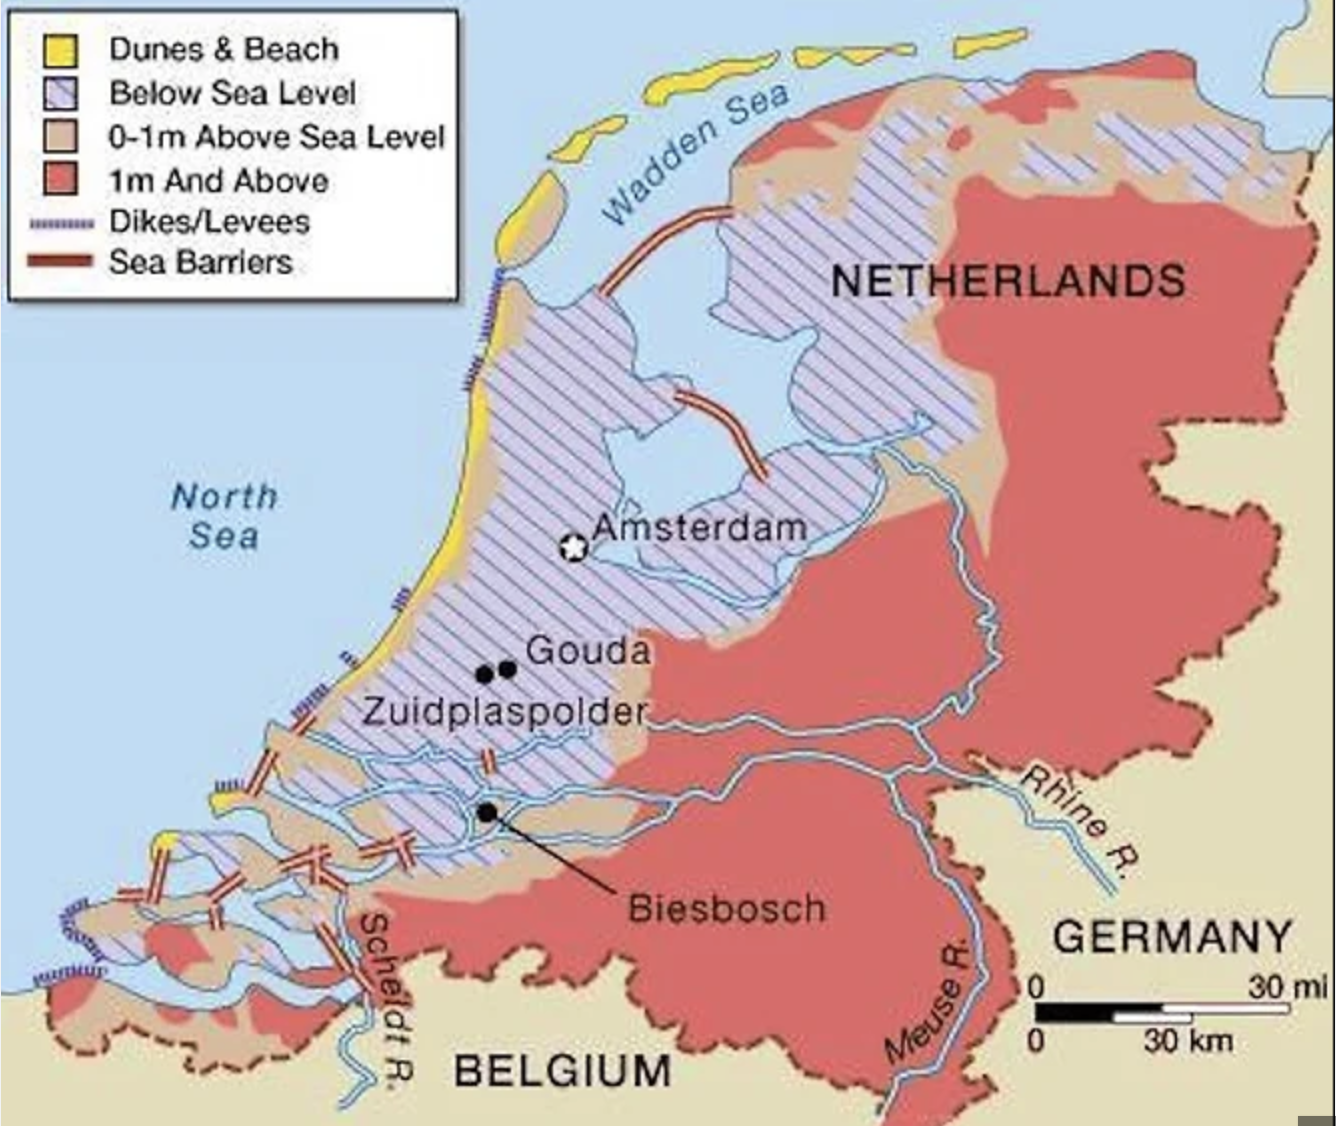
\includegraphics[width=0.85\linewidth]{figures/deltaDam.png}
\end{figure}
\end{frame}

%\begin{frame}{Other motivating examples}
%\begin{itemize}
%\item European 2003 heatwaves: Was the hottest summer on record in Europe since at least 1540. European death toll more than 70000 (debated...).
%\item 
%\end{itemize}
%\end{frame}

\begin{frame}{(Some) Application Areas}
%\setbeamercovered{transparent}
% \begin{itemize}[<+->]
\begin{itemize}
    \item \textbf{Environment:} rainfall, temperatures, snowfall (avalanches), river levels, sea levels, wind speed, pollution, etc.
    \item \textbf{Seismology:} large earthquakes and tsunamis
    \item \textbf{Finance:} financial time series and (re-)insurance
    \item \textbf{Material science:} strength of materials and structures
    \item \textbf{Athletics:} record times
\end{itemize}
\end{frame}

}




{
\section{Block Maxima Approach}



\begin{frame}{Recall Central Limit Theorem}
%\setbeamercovered{transparent}
% \begin{itemize}[<+->]
\begin{itemize}
    \item Suppose that \( Y, Y_1, Y_2, \ldots \) is a sequence of i.i.d. non-degenerate random variables defined with distribution \( F(y) \).

    \item The i.i.d. assumption may be slightly relaxed...

    \item We define the partial sums as:
    \[
    S_0 = 0, \quad S_n = Y_1 + \cdots + Y_n, \quad n \geq 1,
    \]
    
    \item And the arithmetic (or sample) means:
    \[
    \overline{Y}_n = \frac{S_n}{n}, \quad n \geq 1.
    \]
    \item If \(\sigma^2 = \text{var}(Y) < \infty\), then as \(n \to \infty\):
    \[
    Z_n = \left( n^{-1/2} \sigma \right)^{-1} (\overline{Y}_n - \mu) \xrightarrow{D} Z \sim \mathcal{N}(0, 1),
    \]
    where \(\mu = E(Y)\) and \(\mathcal{N}(0, 1)\) is the standard normal distribution.


\end{itemize}

\end{frame}


{\subsection{Extremal Types Theorem: GEV Distribution}

\begin{frame}{Maxima I}
Would like to have a result similar to the CLT, but for extremes (minima/maxima)...
%\setbeamercovered{transparent}
% \begin{itemize}[<+->]
\begin{itemize}
    \item We start by assuming that $Y, Y_1, Y_2, \ldots$ is a sequence of i.i.d. (non-degenerate) random variables with distribution $F(y)$.
    \item The i.i.d. assumption may be generalized for non-stationary extremes and accounting for temporal dependence.
    \item We define the partial (or sample) maximum as
    \[
    M_n = \max(Y_1, \ldots, Y_n).
    \]
    \item The following theory also applies to minima because
    \[
    \min(Y_1, \ldots, Y_n) = -\max(-Y_1, \ldots, -Y_n).
    \]
    \item Our general discussion is for maxima, and we make this transformation without comment when we model minima.
\end{itemize}
\end{frame}


\begin{frame}{Maxima II}
%\setbeamercovered{transparent}
% \begin{itemize}[<+->]
\begin{itemize}
    \item The distribution function of the sample maximum $M_n$ is
\begin{align*}
    \Pr(M_n \leq y) &= \Pr(Y_1 \leq y, \ldots, Y_n \leq y) \\ &=  \Pr(Y_1 \leq y) \times \cdots \times \Pr(Y_n \leq y) = F^n(y).
  \end{align*}
    \item $F$ is typically unknown, so we need to approximate $F^n$ by some limit distribution.
    \item What distributions can arise? As $n \to \infty$, one has
    \[
    F^n(y) \to
    \begin{cases}
        0, & \text{if } F(y) < 1, \\
        1, & \text{if } F(y) = 1,
    \end{cases}
    \]
    so $M_n \xrightarrow{D} y_F$, where $y_F = \sup\{y : F(y) < 1\}$ is the upper support point of $F$. Hence, the limit distribution is degenerate!
    \item \textbf{Intuitively:} As $M_n$ is always increasing with $n$, we should renormalize to get a non-degenerate limiting distribution!
\end{itemize}
\end{frame}

\begin{frame}{Maxima III}
We seek to mimic the Central Limit Theorem...
%\setbeamercovered{transparent}
 %\begin{itemize}[<+->]
 \begin{itemize}
    \item We will investigate limiting distributions for renormalized maxima
    \[
    M^*_n = a_n^{-1} (M_n - b_n),
    \]
    for some suitable sequences of constants $a_n > 0$ and $b_n \in \mathbb{R}$.
    \item Question: What kind of limiting distributions can arise for $M^*_n$, as $n \to \infty$?
    \item The distribution of $M^*_n$ is
    \begin{align*}
    \Pr(M^*_n \leq y) &= \Pr\left\{a_n^{-1} (M_n - b_n) \leq y\right\} \\
    &= \Pr(M_n \leq a_n y + b_n) \\
    &= F^n(a_n y + b_n) \\
    &= F^n(u_n) \\ &= \Pr(M_n \leq u_n),
 \end{align*}
    where $u_n$ is a suitable threshold sequence.
\end{itemize}
\end{frame}


\begin{frame}{Back to Affine Transformations}
Let's assume that a threshold sequence $u_n$ exists.
%\setbeamercovered{transparent}
% \begin{itemize}[<+->]
\begin{itemize}
    \item We will focus on sequences of the type $u_n = a_n y + b_n$ (affine transformation).
    \item This choice is simple, mimics the CLT, and allows us to get non-degenerate limits for a wide family of distributions.
    \item Questions:
    \begin{itemize}
        \item How to choose $a_n$ and $b_n$? Is the choice unique?
        \item What distributions arise as limits for $M^*_n = a_n^{-1} (M_n - b_n)$ (properly renormalized)?
        \item If there are several limit distributions, how to characterize their \textbf{``max-domains of attraction"}? 
        \item What is the speed of convergence to the limit?
    \end{itemize}
    \item Similarly to the CLT, the notion of max-stability is crucial to start answering these questions.
\end{itemize}

\end{frame}

\begin{frame}{Extremal Types Theorem --  Fisher and Tippett, 1928}
%The distributions $G$ and $G^*$ are said to be of the same type if there are constants $a > 0$ and $b$ such that $G^*(ay + b) = G(y)$ for all $y$.
%\setbeamercovered{transparent}
% \begin{itemize}[<+->]
\begin{itemize}
    \item Let $Y, Y_1, Y_2, \ldots$ be a sequence of i.i.d. random variables. If there exist sequences of constants $a_n > 0$ and $b_n$ such that, as $n \to \infty$,
    \(
    \Pr(M^*_n \leq y) = \Pr\left\{\frac{M_n - b_n}{a_n} \leq y\right\} \to G(y)
    \)
    for some non-degenerate distribution $G$, then $G$ has the same type as one of the following distributions:
    \begin{itemize}
        \item \textbf{I — Gumbel}: $G(y) = \exp\{-\exp(-y)\}$, $-\infty < y < \infty$;
        \item \textbf{II — Fréchet}:
        \(
        G(y) =
        \begin{cases}
        0, & y \leq 0, \\
        \exp(-y^{-\alpha}), & y > 0, \alpha > 0;
        \end{cases}
        \)
        \item \textbf{III — Weibull}:
        \(
        G(y) =
        \begin{cases}
        \exp\{-( -y)^\alpha\}, & y < 0, \alpha > 0, \\
        1, & y \geq 0.
        \end{cases}
        \)
    \end{itemize}
    \item Conversely, each of these $G$'s may appear as a limit for the distribution of $(M_n - b_n)/a_n$, and does so when $G$ itself is the distribution of $Y$.
\end{itemize}

\end{frame}

\begin{frame}{Generalized Extreme-Value (GEV) Distribution}
This family encompasses all three of the previous extreme-value limit families:
\[
G(y) = \exp \left\{
-\left[1 + \xi \left(\frac{y - \mu}{\sigma}\right)\right]^{-1/\xi}_+
\right\},
\]
defined on $\{y : 1 + \xi(y - \mu)/\sigma > 0\}$. Here, $a_+ = \max(0, a)$.

%\setbeamercovered{transparent}
% \begin{itemize}[<+->]
\begin{itemize}
    \item $\mu$ is a location parameter, while $\sigma > 0$ is a scale parameter.
    \item $\xi$ is a shape parameter determining the rate of tail decay, with
    \begin{itemize}
        \item $\xi > 0$ giving the heavy-tailed (Fréchet) case,
        \item $\xi = 0$ (interpreted as $\xi \to 0$) giving the light-tailed (Gumbel) case,
        \item $\xi < 0$ giving the short-tailed (reversed Weibull) case.
    \end{itemize}
    \item If $Y \sim \text{GEV}(\mu, \sigma, \xi)$, one has $E(Y^r) < \infty \iff \xi r < 1$.
    \item By the Extremal Types Theorem (ETT), the GEV distribution is the only univariate max-stable distribution.
\end{itemize}


\end{frame}

\begin{frame}{Examples: Limit Laws for Maxima}
%\setbeamercovered{transparent}
% \begin{itemize}[<+->]
\begin{itemize}
   \item \textbf{Uniform distribution}: Maxima from the Uniform distribution $F(y) = \frac{y}{\theta}$, $y \in (0, \theta)$, $\theta > 0$, are “attracted” to the reversed Weibull distribution.
    \item \textbf{Gaussian distribution}: Maxima from the Gaussian distribution $F(y) = \Phi(y)$, $y \in \mathbb{R}$, are “attracted” to the Gumbel distribution.
    \item \textbf{Exponential distribution}: Maxima from the Exponential distribution $F(y) = 1 - \exp(-\theta y)$, $y > 0$, $\theta > 0$, are “attracted” to the Gumbel distribution.
    \item \textbf{Pareto distribution}: Maxima from the Pareto distribution $F(y) = 1 - y^{-\alpha}$, $y > 1$, $\alpha > 0$, are “attracted” to the Fréchet distribution.
    \item \textbf{Cauchy distribution}: Maxima from the Cauchy distribution $F(y) = \frac{1}{2} + \frac{1}{\pi} \arctan(y)$, $y \in \mathbb{R}$, are “attracted” to the Fréchet distribution.
\end{itemize}
\end{frame}

\begin{frame}{Statistical Inference -- Basic Idea}

Suppose we have a time series of daily values $Y_1, Y_2, \ldots$ supposed to be independent and identically distributed from some distribution $F$.

%\setbeamercovered{transparent}
% \begin{itemize}[<+->]
\begin{itemize}
    \item Extract maxima $M_n = \max(Y_1, \ldots, Y_n)$ of blocks of the original series:
    \begin{itemize}
        \item For environmental time series, typically $n = 365$ for annual maxima, $n = 30$ for monthly maxima.
        \item In finance, typically $n = 250$ for annual maxima, $n = 20$ for monthly data.
    \end{itemize}
    \item Assume the resulting series of maxima $Z_1, \ldots, Z_N$, where $Z_j$ is the maximum of the $j$th block of $n$ consecutive observations, is distributed according to the GEV distribution $G(z)$ for some parameters $\mu, \sigma, \xi$.
    \item Estimate the unknown parameters and use the fitted GEV model to make extrapolations.
\end{itemize}

\end{frame}

}

{\subsection{Likelihood Estimation, Quantile and Return Levels}
\begin{frame}{Quantiles and return levels}
%\setbeamercovered{transparent}
% \begin{itemize}[<+->]
\begin{itemize}
    \item Let $0 < p < 1$ denote the “excess probability” and define
    \[
    z_p = G^{-1}(1 - p) = \mu + \frac{\sigma}{\xi} \left[ \{-\log(1 - p)\}^{-\xi} - 1 \right],
    \]
    or equivalently: $1 - G(z_p) = p$.
    \item The level $z_p$ is called the return level associated with the return period $1/p$.
    \item If the $\text{GEV}(\mu, \sigma, \xi)$ distribution $G$ is used to model annual maxima, the $M$-year return level (with return period $M$) is simply
    \[
    z_{1/M} = Q(M) = G^{-1}(1 - 1/M).
    \]
    \item Interpretation: “The $M$-year return level is exceeded (on average) once every $M$ years.”
    \item Provides a way to extrapolate to higher quantiles than the observed maximum (i.e., very small $p$) based on theoretically justified arguments.
    \item Depend on unknown parameters $\Rightarrow$ Need to be estimated from the data!
\end{itemize}
\end{frame}

\begin{frame}{Likelihood Estimation -- GEV Distribution}
 \footnotesize
%\setbeamercovered{transparent}
% \begin{itemize}[<+->]
\begin{itemize}
    \item \textbf{Log likelihood function for GEV distribution:}
    \begin{align*}
    \ell(\mu, \sigma, \xi) = \sum_{i=1}^{N} \left[ -\log \sigma - \left(1 + \frac{1}{\xi}\right) \log \left\{1 + \xi \frac{z_i - \mu}{\sigma}\right\} - \left\{1 + \xi \frac{z_i - \mu}{\sigma}\right\}^{-1/\xi} \right].
      \end{align*}
    Note: This equals $-\infty$ if any $1 + \xi \frac{z_i - \mu}{\sigma} < 0$.
    
    \item \textbf{Numerical maximization of log likelihood.}
    
    \item \textbf{Calculation of standard errors from inverse of observed information matrix (also obtained numerically).}
    
    \item \textbf{Diagnostic checks:}
    \begin{itemize}
        \item Probability plots
        \item Quantile plots
        \item Return level plots
    \end{itemize}
    
    \item \textbf{Comparison of competing models:}
    \begin{itemize}
        \item Nested models through deviance (likelihood ratio statistic)
        \item Non-nested models by minimizing the Akaike information criterion (AIC):
        \[
        \text{AIC} = -2\ell(\hat{\theta}) + 2p,
        \]
        (or similar criteria)
    \end{itemize}
    
    \item \textbf{Calculation of confidence intervals for return levels using profile log likelihood.}
\end{itemize}

\end{frame}



\begin{frame}{Regularity of MLE}
\footnotesize
%\setbeamercovered{transparent}
% \begin{itemize}[<+->]
\begin{itemize}
    \item \textbf{Usual regularity conditions for validity of conventional likelihood inference:}
    \begin{itemize}
        \item Require that the support of the density does not depend on the parameter values.
        \item \textbf{Not the case for the GEV!}
    \end{itemize}

    \item The score statistic \( U(\theta) = \frac{\partial \ell(\theta)}{\partial \theta} \) must have finite first and second moments that satisfy:
    \[
    \text{var}\left( \frac{\partial \ell(\theta)}{\partial \theta} \right) = E\left\{ -\frac{\partial^2 \ell(\theta)}{\partial \theta \partial \theta^T} \right\}.
    \]

    \item For the GEV, the \(r\)th moment of the score only exists if \( r\xi > -1 \) (exercise!).

    \item Smith (1985) established that the limiting behavior of the MLE depends on the value of the shape parameter \(\xi\):
    \begin{itemize}
        \item \(\xi > -1/2\): MLE obeys standard theory;
        \item \(-1 < \xi \leq -1/2\): MLE is a solution to the score equation, but does not have the usual limiting distribution;
        \item \(\xi \leq -1\): MLE is not even a solution to the score equation.
    \end{itemize}

    \item In most environmental problems, we find \(\hat{\xi} \approx 0\) so can use MLE.

    \item Penalized likelihood methods (see exercise) or Bayesian inference can be used to force \(|\xi| < 1/2\).
\end{itemize}

\end{frame}

}


}

{
\section{Peak-Over-Threshold (POT) Approach}
\begin{frame}{Issue With the Block Maxima Approach}
%\setbeamercovered{transparent}
% \begin{itemize}[<+->]
\begin{itemize}
    \item The annual maxima method can be inefficient if more data are available (as we keep only one observation per year).

    \item One solution: Take smaller blocks... But:
    \begin{itemize}
        \item Loose interpretation if blocks do not correspond to natural cycles...
        \item What does it mean to consider blocks of 53 days of observations, say?
        \item Weekly or monthly blocks?
        \begin{itemize}
            \item Sometimes too small for asymptotic model to be valid.
        \end{itemize}
    \end{itemize}

    \item Alternatives?
    \begin{itemize}
        \item Peaks-Over-Thresholds (POT) method
        \item \(r\)-largest order statistics method (not covered here)
    \end{itemize}

    \item Both are special cases of a point process representation (not covered here), under which we use a Poisson process to approximate the occurrence of those values that exceed a (high) threshold.
\end{itemize}

\end{frame}

\begin{frame}{Comments}
\begin{itemize}
    \item The fixed number of annual maxima has been replaced by a random number of exceedances over the threshold.
    \begin{itemize}
        \item We now have more observations in the tail of the distribution.
    \end{itemize}

    \item Dependence in the underlying series means that exceedances occur in clusters, which we may need to model (but we will not cover this aspect here and assumed independence throughout).

    \item For now, we suppose that the underlying series comprises independent identically distributed (i.i.d.) observations, whose maxima have a non-degenerate limit after renormalization.
\end{itemize}
\end{frame}


{\subsection{Pickands–Balkema–de Haan Theorem: GP Distribution}

\begin{frame}{Generalized Pareto (GP) Distribution}
\begin{figure}
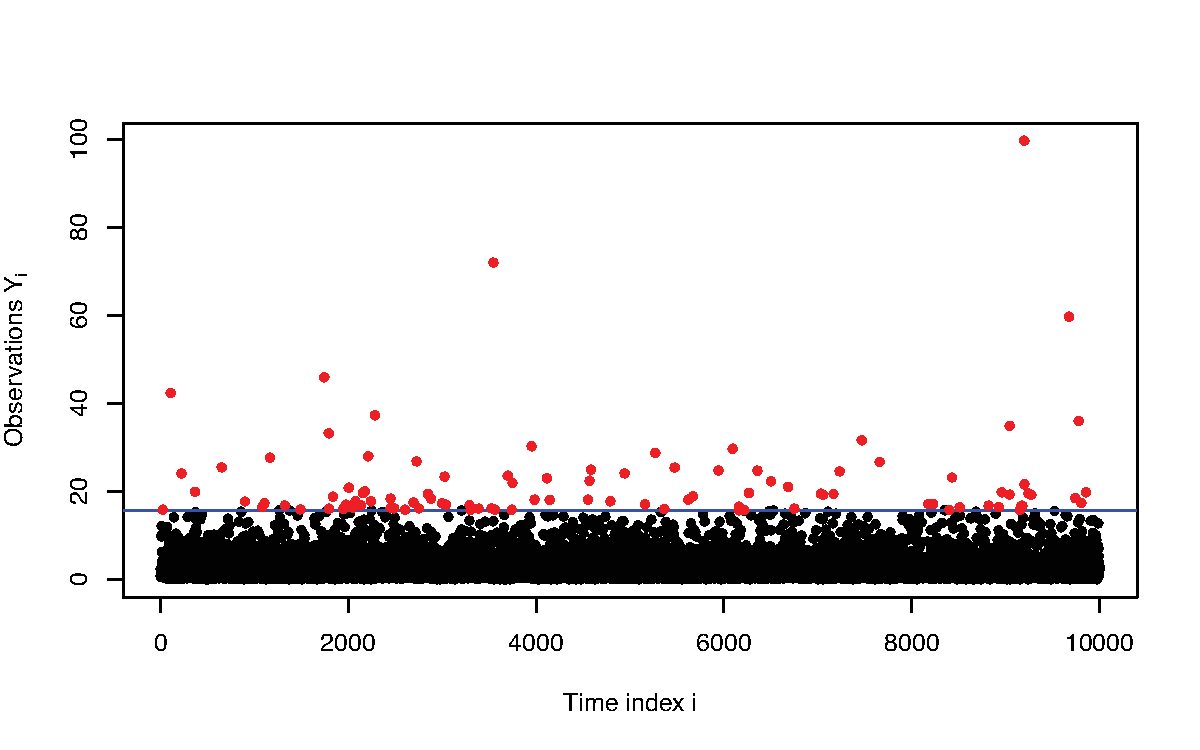
\includegraphics[scale=0.5]{figures/Plot2b.eps}
\end{figure}
\end{frame}


\begin{frame}{Pickands–Balkema–de Haan Theorem}
%\setbeamercovered{transparent}
% \begin{itemize}[<+->]
\begin{itemize}
 \item In extreme value theory {\color{violet} generalized Pareto (GP)} distribution plays a key role in the peaks-over-threshold (POT) approach  and is the only possible limit for the marginal distribution of appropriately rescaled threshold exceedances. 
    \item Provides a justification for fitting the generalized Pareto (GP) distribution to high threshold exceedances:
    \[
    Y - u \mid Y > u \overset{d}{\sim} 1 - \left(1 + \xi \frac{y}{a(u)}\right)^{-1/\xi}, \quad \text{for large } u,
    \]
    where \(\xi\) is the shape parameter and \(a(u)\) is a scaling function dependent on the threshold \(u\).
\end{itemize}
\end{frame}


\begin{frame}{Generalized Pareto (GP) distribution)}
\begin{itemize}
    \item The GP\((\tau, \xi)\) is defined as:
    \[
    H(y) =
    \begin{cases} 
        1 - \left(1 + \xi \frac{y}{\tau}\right)^{-1/\xi}, & \xi \neq 0, \\
        1 - \exp\left(-\frac{y}{\tau}\right), & \xi = 0
    \end{cases}
    \]

    \item \(\tau > 0\) is the scale parameter, \(\xi \in \mathbb{R}\) is the shape parameter.

        \item \textbf{Special cases:}
        \begin{itemize}
            \item \(\xi > 0\): Power-law. For $\xi=1$ standard Pareto distribution
            \item \(\xi = 0\): Exponential
            \item \(\xi < 0\): Upper bounded. For \(\xi = -1\): Uniform distribution 
        \end{itemize}
\end{itemize}
\vspace{-7mm}
\begin{figure}
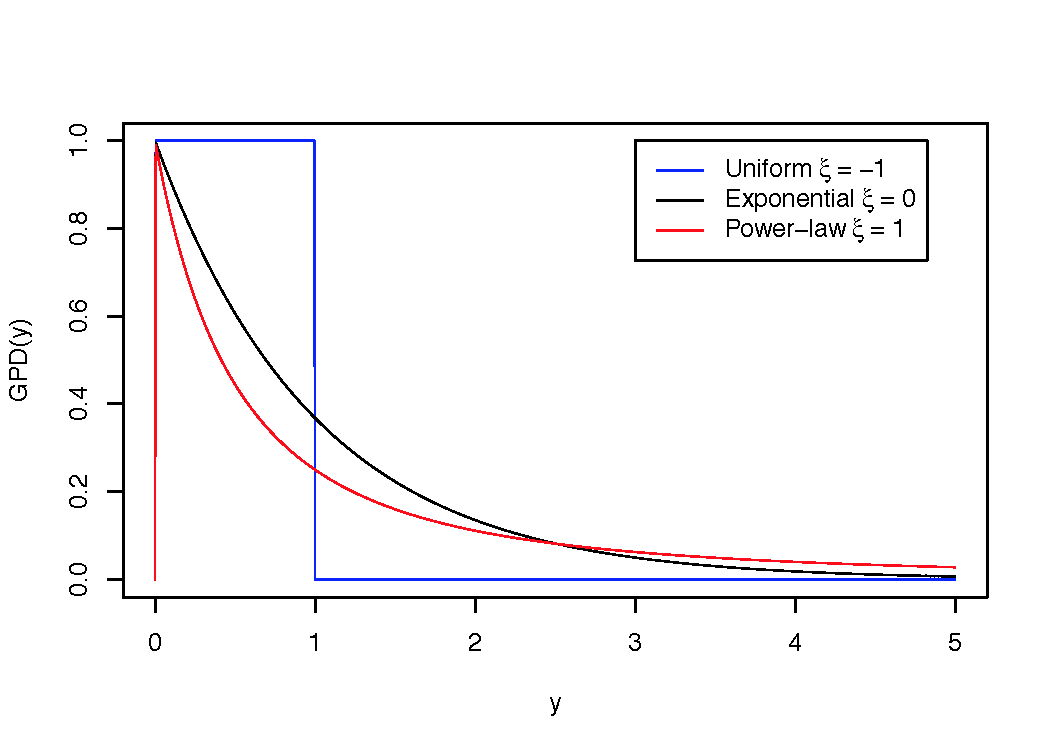
\includegraphics[scale=0.35]{figures/Plot4.eps}
\end{figure}
\end{frame}



\begin{frame}{Generalized Pareto (GP) Distribution}
%\setbeamercovered{transparent}
% \begin{itemize}[<+->]
\begin{itemize}
    \item \textbf{Uniform distribution}:  For the \(\text{Unif}(0, 1)\) distribution, with \(F(y) = y\), \(y \in [0, 1]\) properly renormalized exceedances over high thresholds converge in distribution to a GP distribution with \(\xi = -1\).
    
    \item \textbf{Exponential distribution:} For the \(\text{Exp}(\lambda)\) distribution, with \(F(y) = 1 - \exp(-\lambda y)\), \(y > 0, \lambda > 0\), properly renormalized exceedances over high thresholds converge in distribution to a GP distribution with \(\xi = 0\).
  
    \item \textbf{Pareto distribution} For the \(\text{Pareto}(\alpha)\) distribution, with \(F(y) = 1 - y^{-\alpha}\), \(y > 1, \alpha > 0\), properly renormalized exceedances over high thresholds converge in distribution to a GP distribution with \(\xi = 1/\alpha > 0\).

    \item Under the same conditions on \(\xi\) as for the GEV, the GP distribution has finite moments and is regular for likelihood inference.
\end{itemize}
\end{frame}

{\subsection{Likelihood Estimation, Quantile and Return Levels}
\begin{frame}{Likelihood estimation -- POT approach (GP distribution)}
%\setbeamercovered{transparent}
% \begin{itemize}[<+->]
\begin{itemize}
    \item Choose a high threshold \( u \), ensuring that the exceedances above \( u \) are well approximated by a GP distribution.
    \item The GP distribution likelihood is
    \[
    L(\tau, \xi) = \prod_{i=1}^{N_u} \frac{1}{\tau} \left( 1 + \xi \frac{y_i - u}{\tau} \right)^{-1/\xi - 1}_{+},
    \]
    where \( y_1, \ldots, y_{N_u} \) is an enumeration of points exceeding the threshold \( u \).

    \item \(\xi\) is the same as for maxima, but \(\tau = \sigma + \xi(u - \mu)\) (\(\tau\) depends on \( u \))!
    \item Only two parameters (\(\tau, \xi\))? If not, what is the 3rd parameter?
    \begin{itemize}
        \item Probability of exceedance \(\zeta_u = \Pr(Y > u)\).
    \end{itemize}

    \item Numerical maximization of GP distribution (log) likelihood is needed to obtain MLEs \(\hat{\tau}, \hat{\xi}\).
    \item The MLE for \(\zeta_u\) is simply obtained as \(\hat{\zeta}_u = \frac{N_u}{n}\) (as \(N_u \sim \text{Bin}(n, \zeta_u)\)).
\end{itemize}

\end{frame}



\begin{frame}{Quantile and Return Levels}

%\setbeamercovered{transparent}
% \begin{itemize}[<+->]
\begin{itemize}
    \item \textbf{Return Levels for GP distribution:}
    \begin{itemize}
        \item Return level \( z_N \) for an \(N\)-year period when data is observed on a daily scale.
        \item For a given exceedance probability \( p = \frac{1}{365N} \):
        \[
        z_N = 
        \begin{cases}
            u + \frac{\tau}{\xi} \left( \left( \frac{1}{365N} \right)^{-\xi} - 1 \right), & \xi \neq 0, \\
            u - \tau \log \left( \frac{1}{365N} \right), & \xi = 0
        \end{cases}
        \]
        where \( u \) is the threshold, \( \tau \) is the scale parameter, and \( \xi \) is the shape parameter.
    \end{itemize}
    \item \textbf{Interpretation:}
    \begin{itemize}
        \item The \(N\)-year return level \( z_N \) represents the value expected to be exceeded on average once every \(N\) years.
        \item For example, a 100-year return level is the value expected to be exceeded once every 100 years.
    \end{itemize}
\end{itemize}

\end{frame}
}
}

{\section{Recap}
\begin{frame}{Block Maxima Approach}
\begin{itemize}
    \item \textbf{Generalized Extreme Value (GEV) Distribution}
    \begin{itemize}
        \item \textbf{Definition:}
        \begin{itemize}
            \item Distribution function: 
            \[
            G(z; \mu, \sigma, \xi) =
            \begin{cases}
                \exp\left\{ -\left[1 + \xi\left(\frac{z - \mu}{\sigma}\right)\right]^{-1/\xi} \right\}, & \text{if } \xi \neq 0, \\
                \exp\left\{ -\exp\left(-\frac{z - \mu}{\sigma}\right) \right\}, & \text{if } \xi = 0.
            \end{cases}
            \]
        \end{itemize}
        
        \item \textbf{Special Cases:}
        \begin{itemize}
            \item \(\xi = 0\): Gumbel distribution
            \item \(\xi > 0\): Fréchet distribution
            \item \(\xi < 0\): Weibull distribution
        \end{itemize}
        
        \item \textbf{Log-Likelihood Function:}
       For \(N\) observations \(z_1, \ldots, z_N\):
            \[
            \ell(\mu, \sigma, \xi) = -\frac{\log \sigma} {N^{-1}}
            - 
            \sum_{i=1}^{N}\left\{ \left(1 + \frac{1}{\xi}\right)  \log \left(1 + \xi \frac{z_i - \mu}{\sigma}\right)
            + \left(1 + \xi \frac{z_i - \mu}{\sigma}\right)^{-\frac{1}{\xi}}\right\}.
            \]
       
        
        \item \textbf{Parameter Estimation:}
        \begin{itemize}
            \item Parameters \((\mu, \sigma, \xi)\) estimated via Maximum Likelihood Estimation (MLE).
        \end{itemize}
        
        \item \textbf{Model Diagnostics:}
        \begin{itemize}
            \item Use probability plots and return level plots to assess model fit.
        \end{itemize}
    \end{itemize}
\end{itemize}

\end{frame}


\begin{frame}{POT Approach}
\begin{itemize}
    \item \textbf{Generalized Pareto (GP) Distribution}
    \begin{itemize}
        \item \textbf{Definition:}
        \begin{itemize}
            \item Distribution function: 
            \[
            H(y; \tau, \xi) =
            \begin{cases}
                1 - \left(1 + \xi \frac{y}{\tau}\right)^{-1/\xi}, & \text{if } \xi \neq 0, \\
                1 - \exp\left(-\frac{y}{\tau}\right), & \text{if } \xi = 0.
            \end{cases}
            \]
            \item \(\tau > 0\) is the scale parameter, \(\xi \in \mathbb{R}\) is the shape parameter.
        \end{itemize}
        
        \item \textbf{Special Cases:}
        \begin{itemize}
            \item \(\xi = 0\): Exponential distribution
            \item \(\xi > 0\): Pareto distribution
            \item \(\xi < 0\): Bounded distribution
        \end{itemize}
        
        \item \textbf{Log-Likelihood Function:}
         For \(N_u\) exceedances \(y_1, \ldots, y_{N_u}\) over threshold \(u\):
            \[
            \ell(\tau, \xi) = - \frac{\log \tau}{N_u^{-1}} 
            - 
            \sum_{i=1}^{N_u} \left\{\left(1 + \frac{1}{\xi}\right)  \log \left(1 + \xi \frac{y_i - u}{\tau}\right)
            + \left(1 + \xi \frac{y_i - u}{\tau}\right)^{-\frac{1}{\xi}}\right\}.
            \]
        
        \item \textbf{Parameter Estimation:}
        \begin{itemize}
            \item Parameters \((\tau, \xi)\) estimated via MLE.
        \end{itemize}
        
        \item \textbf{Model Diagnostics:}
        \begin{itemize}
            \item Probability plots, return level plots, and evaluate the threshold choice.
        \end{itemize}
    \end{itemize}
\end{itemize}
\end{frame}


}

{
\section{Practical Examples Using R for IID Data}

\begin{frame}{Extreme Value Analysis in R for IID Data}

\begin{itemize}
\item See the code \href{https://github.com/yadavrishikesh/Intro-EVT}{EVT.Rmd} for the detailed study of extreme of precipitation data from western England using both block maxima approach and peaks over threshold approach  
\item Also see the code \href{https://github.com/yadavrishikesh/Intro-EVT}{EVT-synthetic.Rmd} for the application to synthetic data to verify the the max-domain of attractions for few of the standard distributions
\end{itemize}
\textbf{Exercises}
\begin{itemize}
\item Fit the block maxima approach to monthly maxima data. What differences you observed?
\item Fit the threshold approach by changing the thresholds levels. What did you notice? 
\end{itemize}
\end{frame}
}


{\section{Non-Stationary Extremes}
{\subsection{Block Maxima Approach}


\begin{frame}{Regression Models for Extremes}
%\setbeamercovered{transparent}
% \begin{itemize}[<+->]
\begin{itemize}
    \item Classical regression models are useful to describe non-stationarity in the mean.
    \item Usually fitted by least squares (thanks to their optimality properties):
    \begin{itemize}
        \item Identical to MLE under normality;
        \item Best Linear Unbiased Estimator (BLUE) under broad assumptions.
    \end{itemize}
    \item But:
    \begin{itemize}
        \item What if noise is not normal?
        \begin{itemize}
            \item LSE is not the MLE, so not fully efficient as \(n \to \infty\).
        \end{itemize}
        \item What if noise has heavy tails?
        \begin{itemize}
            \item LSE is sensitive to outliers, and increasingly inefficient as the tail becomes heavier.
        \end{itemize}
        \item What if mean is not finite?
        \begin{itemize}
            \item LSE does not work! (to estimate an infinite mean...)
        \end{itemize}
        \item How to use the fitted curve to compute return levels?
    \end{itemize}
\end{itemize}

\end{frame}



\begin{frame}{Regression Models for Maxima}
\footnotesize
%\setbeamercovered{transparent}
% \begin{itemize}[<+->]
\begin{itemize}
    \item By analogy with classical linear regression models, we can deal with non-stationary effects by including covariates into the usual extreme-value parameters.
    \item A suitable model for block maxima \(Z_1, \ldots, Z_N\) may therefore be expressed as
    \[
    Z_i \overset{\text{ind}}{\sim} \text{GEV}(\mu_i, \sigma_i, \xi_i),
    \]
    \[
    \begin{cases}
    \mu_i = \mu(x_i; \beta_\mu) \\
    \sigma_i = \sigma(x_i; \beta_\sigma) > 0 \\
    \xi_i = \xi(x_i; \beta_\xi)
    \end{cases}
    \]
    where \(\mu(x_i; \beta_\mu)\), \(\sigma(x_i; \beta_\sigma) > 0\), and \(\xi(x_i; \beta_\xi)\) are functions of a vector of covariates \(x_i\) and associated vectors of parameters \(\beta_\mu\), \(\beta_\sigma\), \(\beta_\xi\) measuring the effect of covariates.
    \item For example, possible parametric models that depend on time \(t\) could be
    \[
    \begin{aligned}
    \mu_i &= \beta_{\mu 0} + \beta_{\mu 1} (t_i - t_0) \\
    \sigma_i &= \exp \left\{ \beta_{\sigma 0} + \beta_{\sigma 1} (t_i - t_0) \right\} \\
    \xi_i &=
    \begin{cases}
    \beta_{\xi 0}, & t_i < t^\star \\
    \beta_{\xi 1}, & t_i \geq t^\star
    \end{cases}
    \end{aligned}
    \]
    where \(t_0\) is a reference point in time and \(t^\star\) is a change point.
\end{itemize}

\end{frame}


\begin{frame}{Modeling Global Temporal Trends and Seasonality}
%\setbeamercovered{transparent}
% \begin{itemize}[<+->]
\begin{itemize}
    \item Global temporal trends can be modeled as a low-order polynomial:
    \[
    \mu_i = \beta_{\mu 0} + \sum_{q=1}^{Q} \beta_{\mu q} (t_i - t_0)^q, \quad
    \sigma_i = \ldots, \quad \xi_i = \ldots,
    \]
    where \(Q\) is the polynomial order (usually \(Q = 0\) or \(Q = 1\)).

    \item Seasonality (i.e., periodic effects) can be addressed by including harmonic terms. For example, in modeling monthly temperature maxima, one might use:
    \[
    \mu_i = \beta_{\mu 0} + \sum_{k=1}^{K} \left( \beta_{\mu, 2k-1} \sin\left(\frac{2k\pi t_i}{12}\right) + \beta_{\mu, 2k} \cos\left(\frac{2k\pi t_i}{12}\right) \right),
    \]
    where \(t_i\) indicates the month (1–12).

    \begin{itemize}
        \item The divisor 12 ensures yearly periodicity for monthly data, and it can be modified according to the periodicity of the data.
        \item \(K\) determines the number of harmonic terms and is usually kept small for parsimony.
    \end{itemize}
     \item Of course, one may combine seasonal terms, trends, and other covariates.
\end{itemize}

\end{frame}

\begin{frame}{Modeling Considerations for Extremes}
Parsimony is important, especially when dealing with extremes.
%\setbeamercovered{transparent}
% \begin{itemize}[<+->]
\begin{itemize}
    \item Always compare the number of parameters to estimate with the ``effective" number of data available (i.e., \(N\) maxima).
    \item The shape parameter \(\xi\) is especially difficult to estimate (i.e., with high uncertainty), so it is common to keep it constant:
    \[
    \xi_i = \xi(x_i; \beta_\xi) = \beta_{\xi 0}, \quad i = 1, \ldots, N.
    \]
    \item Often in practice, \(\sigma \propto \mu\), so it might make sense to fit a model where:
    \[
    \sigma(x_i; \beta_\sigma) = c \times \mu(x_i; \beta_\mu), \quad i = 1, \ldots, N,
    \]
    and \(c\) is a constant to estimate.
\end{itemize}

\end{frame}


\begin{frame}{Estimation and Diagnostics}
\begin{itemize}
    \item Estimation may be performed by maximum likelihood inference. Let \(g(z; \mu, \sigma, \xi)\) denote the GEV density. The log likelihood may be written as:
   \begin{align*}
    \ell(\beta_\mu, \beta_\sigma, \beta_\xi) &= \sum_{i=1}^{N} \log \left\{ g(z_i; \mu_i, \sigma_i, \xi_i) \right\} \\
    &= -\sum_{i=1}^{N} \log \left\{ \sigma(x_i; \beta_\sigma) \right\}  \\
  & - \sum_{i=1}^{N} \left( 1 + \frac{1}{\xi(x_i; \beta_\xi)} \right) \log \left( 1 + \xi(x_i; \beta_\xi) \frac{z_i - \mu(x_i; \beta_\mu)}{\sigma(x_i; \beta_\sigma)} \right) \\
  & + \sum_{i=1}^{N} \left( 1 + \xi(x_i; \beta_\xi) \frac{z_i - \mu(x_i; \beta_\mu)}{\sigma(x_i; \beta_\sigma)} \right)^{-1/\xi(x_i; \beta_\xi)} .
   \end{align*}
    \item Numerical maximization with respect to the parameters is needed.
    \item Good starting values are essential for successful optimization, especially when the number of parameters is fairly large.
\end{itemize}

\end{frame}





}

{\subsection{POT Approach}
\begin{frame}{Non-Stationary Models for Threshold Exceedances}
\begin{itemize}
    \item Similar techniques are applicable for the POT  models, but threshold selection can be tricky.
    \item Quantile regression may be useful for the choice of non-stationary thresholds.
    \item Let us study an example to illustrate the advantages, drawbacks, and difficulties of non-stationary POT approaches.
\end{itemize}

\end{frame}


\begin{frame}{Non-Stationary Threshold Choice}
%   \setbeamercovered{transparent}
% \begin{itemize}[<+->]
\begin{itemize}
        \item Linear regression:
        \begin{itemize}
            \item Model: \(u_i = \mathbf{x}_i^T \beta + \epsilon_i\), \(\epsilon_i \overset{\text{iid}}{\sim} (0, \sigma^2)\), where \(\mathbf{x}_i\) is a vector of covariates for the \(i\)th observation and \(\beta\) is a vector of unknown parameters.
            \item Fit by least squares: \(\hat{\beta}_2 = \min \sum_{i=1}^{n}(u_i - \mathbf{x}_i \beta)^2\).
            \item \(\mathbf{x}_i^T \hat{\beta}_2\) is an estimate of the conditional mean of \(Y_i\).
        \end{itemize}
        \item \(L_1\) regression: Replace \(L_2\) by \(L_1\) loss function:
        \begin{itemize}
            \item Fit by least absolute deviations: \(\hat{\beta}_1 = \min \sum_{i=1}^{n} |u_i - \mathbf{x}_i \beta|\).
            \item \(\mathbf{x}_i^T \hat{\beta}_1\) is an estimate of the conditional median of \(Y_i\).
        \end{itemize}
        \item Quantile regression: Use “pinball” loss function \(L(\cdot; p_u)\):
        \begin{itemize}
            \item Estimated parameters: \(\hat{\beta}_{p_u} = \min \sum_{i=1}^{n} L(u_i - \mathbf{x}_i \beta; p_u)\), where
            \[
            L(y; \tau) =
            \begin{cases} 
            p_u y, & y \geq 0; \\
            -(1 - p_u) y, & y < 0.
            \end{cases}
            \]
            \item \(\mathbf{x}_i^T \hat{\beta}_{p_u}\) is an estimate of the conditional \(p_u\)-quantile of \(u_i\).
        \end{itemize}
    \end{itemize}
    And so infernce is carried out in two steps;
\begin{itemize}
    \item \textbf{Step 1:} quantile regression to obtain time-varying threshold \(u(t)\).
    \item \textbf{Step 2:} GP distribution model to exceedances \(Y_i - u(t) \mid Y_i > u(t)\).
\end{itemize}

\end{frame}


\begin{frame}{Non-Stationary POT Model - Comments}
%   \setbeamercovered{transparent}
% \begin{itemize}[<+->]
\begin{itemize}
        \item We may let the GP distribution parameters \(\tau_u, \xi\) depend on covariates.
        \item Inference in two steps implies that uncertainty in  \(u(t)\) is neglected.
        \item How to perform model comparisons? Cannot use AIC/BIC when \(u(t)\) is different.
        \item Fit may quite strongly depend on the choice of \(u(t) \Rightarrow\) Bad!
        \item Care needed with model interpretation: with GP(\(\tau_u, \xi\)), change of threshold \(u \to v > u\) changes scale parameter
        \[
        \tau_u \to \tau_v = \tau_u + \xi(v - u).
        \]
        \item So for example, if \(t\) denotes time, and \(x\) denotes another covariate, the model
        \[
        \tau_u = s_1(t), \quad \xi = s_2(x).
        \]
        at threshold \(u\) will become
        \[
        \tau_v = s_1(t) + s_2(x)(v - u), \quad \xi = s_2(x).
        \]
        at threshold \(v > u\). So interpretation depends on threshold: avoid it.
    \end{itemize}

\end{frame}


}


}


{
\section{Practical Examples Using R for non-IID Data}

\begin{frame}{Extreme Value Analysis in R for non-IID Data}

\begin{itemize}
\item See the code \href{https://github.com/yadavrishikesh/Intro-EVT}{EVT-NonStationary.Rmd} for the detailed study of non-stationary extreme of precipitation data from western England using both non-stationary block maxima approach and non-stationary peaks over threshold approach  
\end{itemize}
\textbf{Exercises}
\begin{itemize}
\item Try other models and compare them?
\end{itemize}
\end{frame}
}


\begin{frame}{There is Still Much More...}
\begin{itemize}
\item Univariate extremes
\begin{itemize}
\item point process approach 
\item r-largest order statistics approach
\item extremes of temporally dependent extremes 
\end{itemize}
\item Multivariate extremes 
\item Spatio-temporal modeling of extremes 
\end{itemize}
\end{frame}
%
%\begin{frame}{Plan for Day 2}
%\Huge{R-Keras vs coding your own Neural Networks from scratch?}
%\end{frame}

%\begin{frame}[allowframebreaks]{References}
%  \bibliography{demo}
%  \bibliographystyle{abbrv}
\end{frame}

\end{document}
